\medskip

On considère $f$ la fonction définie sur l'intervalle $]0; +\infty[$ par $f(x) = \dfrac{\e^{\sqrt{x}}}{2 \sqrt{x}}$ et on appelle $C_f$ sa courbe représentative dans un repère orthonormé.

\begin{enumerate}
\item On définit la fonction $g$ sur l'intervalle $]0~;~ +\infty[$ par $g(x) = \e^{\sqrt{x}}$
	\begin{enumerate}
		\item La fonction $g$ est continue et dérivable sur $]0~;~+\infty[$, donc $\forall x \in ]0~;~+\infty[$,

$g'(x) = \dfrac{1}{2\sqrt{x}}\times \e^{\sqrt{x}}= \dfrac{\e^{\sqrt{x}}}{2\sqrt{x}} = f(x)$.
		\item La fonction $f$ est continue et dérivable sur $]0~;~+\infty[$, donc $\forall x \in ]0~;~+\infty[$,
	
$f'(x) = \dfrac{\dfrac{1}{2\sqrt{x}}\e^{\sqrt{x}}\times2\sqrt{x}-\e^{\sqrt{x}}\times 2\dfrac{1}{2\sqrt{x}}}{(2\sqrt{x})^2} = \dfrac{\e^{\sqrt{x}}-\dfrac{\e^{\sqrt{x}}}{\sqrt{x}}}{4x}=\dfrac{\dfrac{\sqrt{x}\e^{\sqrt{x}}-\e^{\sqrt{x}}}{\sqrt{x}}}{4x}= \dfrac{\e^{\sqrt{x}} (\sqrt{x} - 1)}{4 x \sqrt{x}}$.
	\end{enumerate}
	\item 
	\begin{enumerate}
		\item $\ds \lim\limits_{x \to 0} \e^{\sqrt{x}}=1$ et $\ds \lim\limits_{x \to 0} 2\sqrt{x}=0$ avec $\dfrac{\e^{\sqrt{x}}}{2 \sqrt{x}} > 0$ donc $\ds \lim\limits_{x \to 0}f(x)=+\infty$.
		\item Donc $C_f$ admet une asymptote verticale d'équation $x=0$.
	\end{enumerate}
	\item 
	\begin{enumerate}
		\item D'après les croissances comparées, $\ds \lim\limits_{u \to +\infty} \dfrac{\e^u}{u}=+\infty$ donc par composition de limites (en posant $u(x)=\sqrt{x}$) $\lim\limits_{x \to +\infty} f(x)=+\infty$.
		\item $\forall x \in ]0~;~+\infty[$, $\e^{\sqrt{x}}>0$ et $4 x \sqrt{x}>0$ donc $f'(x)$ a le même signe que $\sqrt{x}-1$.

$\sqrt{x}-1\geqslant 0 \iff \sqrt{x}\geqslant1 \iff x\geqslant1$

\begin{center}
	\begin{tikzpicture}
			\tkzTab{$x$ / 1 , $f'(x)$ / 1, $f(x)$ / 1.5}{$0$, $1$, $+\infty$}
			{d, -, z, +, }
			{D+ / $+\infty$, -/ $\dfrac{\e}{2}$, +/ $+\infty$}
	\end{tikzpicture}
\end{center}
		\item La fonction $f$ est continue et strictement croissante sur l'intervalle $[1~;~+\infty[$ à valeurs dans $\left[\dfrac{\e}{2}~;~+\infty\right[$. Or $2\in \left[\dfrac{\e}{2}~;~+\infty\right[$ (car $\dfrac{\e}{2}<2$) donc d'après le corollaire du TVI, l'équation $f(x) = 2$ admet une unique solution notée $\alpha$ dans $[1;+\infty[$.

À la calculatrice : $\alpha\approx 4,6$.
	\end{enumerate}
	\item $I = \ds\int_1^2 f(x) \, \text{d}x$.
	\begin{enumerate}
		\item $\forall x \in [1~;~2]$, $f(x)=\dfrac{\e^{\sqrt{x}}}{2 \sqrt{x}}=\dfrac{1}{2\sqrt{x}} \times {\e^{\sqrt{x}}}$.
En remarquant que la dérivée de la fonction $g$ est la fonction $f$, $g$ est une primitive de $f$.

Donc $I = \ds\int_1^2 f(x) \, dx=\left[g(x)\right]_1^2=\left[\e^{\sqrt{x}}\right]_1^2= \e^{\sqrt{2}}- \e$
		\item L'aire du domaine $\begin{cases} 1\leqslant x \leqslant 2 \\ 0\leqslant y \leqslant f(x)\end{cases}$ est égale à $\e^{\sqrt{2}}- \e$.
		
$I$ est donc l'aire du domaine compris entre $\mathcal{C}_f$ , l'axe des abscisses et les droites d'équation $x =1$ et $x =2$.
	\end{enumerate}
	\item $\forall x \in ]0~;~ +\infty[$, $f''(x) = \dfrac{\e^{\sqrt{x}} (x - 3 \sqrt{x} + 3)}{8 x^2 \sqrt{x}}$
	\begin{enumerate}
		\item On pose $\forall x \in ]0~;~ +\infty[$, $X=\sqrt{x}$.

$x - 3 \sqrt{x} + 3=X^2-3X+3$.

		$\Delta=(-3)^2-4\times 1\times 3=-3<0$ donc $\forall X \in ]0~;~ +\infty[$, $X^2-3X+3>0$ donc $\forall x \in ]0; +\infty[$, $x - 3 \sqrt{x} + 3>0$.
		\item $\forall x \in ]0; +\infty[$, $e^{\sqrt{x}}>0$ et $x - 3 \sqrt{x} + 3>0$ et $8 x^2 \sqrt{x}>0$ donc $f''(x)>0$.
		
		La fonction $f$ est convexe sur $]0~;~ +\infty[$.
	\end{enumerate}
\end{enumerate}
